% define some macros:
\newcommand{\munged}{{\tt munged}}
\newcommand{\srun}{{\tt srun}}
\newcommand{\scancel}{{\tt scancel}}
\newcommand{\squeue}{{\tt squeue}}
\newcommand{\scontrol}{{\tt scontrol}}
\newcommand{\sinfo}{{\tt sinfo}}
\newcommand{\slurmctld}{{\tt slurmctld}}
\newcommand{\slurmd}{{\tt slurmd}}

\maketitle

\begin{abstract}
Simple Linux Utility for Resource Management (SLURM) is an open source,
fault-tolerant, and highly scalable cluster management and job 
scheduling system for Linux clusters of 
thousands of nodes.  Components include machine status, partition
management, job management, scheduling and stream copy modules.  
This paper presents a overview of the SLURM architecture and functionality. 
\end{abstract}

\vspace{0.25in}

%\begin{center}
%
\epsfig{file=slurm.eps,width=4in}
%\end{center}

\newpage

\section{Overview}

SLURM\footnote{A tip of the hat to Matt Groening and creators of {\em Futurama},
where Slurm is the highly addictive soda-like beverage made from worm
excrement.} (Simple Linux Utility for Resource Management) 
is a resource management 
system suitable for use on Linux clusters, large and small.  After 
surveying\cite{Jette2002} resource managers available for Linux and finding 
none that were simple, highly scalable, and portable to different cluster 
architectures and interconnects, the authors set out to design a new system.

The result is a resource management system with the following general
characteristics:

\begin{itemize}
\item {\em Simplicity}: SLURM is simple enough to allow motivated end users
to understand its source code and add functionality.  The authors will 
avoid the temptation to add features unless they are of general appeal. 

\item {\em Open Source}: SLURM is available to everyone and will remain 
free; its source code is distributed under the GNU General Public 
License\cite{GPL2002}.

\item {\em Portability}: SLURM is written in the C language, with a GNU 
{\em autoconf} configuration engine.  SLURM also supports a {\em plug-in} 
mechanism, which permits a variety of different infrastructures to be 
easily supported. The SLURM configuration file specifies which set of 
plug-in modules should be used. While initially written for Linux, other 
UNIX-like operating systems should be easy porting targets.

\item {\em Interconnect independence}: SLURM supports UDP/IP based
communication and the Quadrics Elan3 interconnect.  Adding support for 
other interconnects, including topography constraints, is straightforward 
and will utilize the plug-in mechanism described above\footnote{SLURM 
presently requires the specification of interconnect at build time}.

\item {\em Scalability}: SLURM is designed for scalability to clusters of
thousands of nodes. The SLURM controller for a cluster with 1000 nodes 
occupies on the order of 2 MB of memory and excellent performance has 
been demonstrated. Jobs may request a range of nodes, potentially 
permitting faster initiation than otherwise possible.

\item {\em Fault tolerance}: SLURM can handle a variety of failure modes
without terminating workloads, including crashes of the node running 
the SLURM controller. 
User jobs may be configured to continue execution despite the failure 
of one or more nodes. 
The user command controlling a job, {\tt srun}, may detach and reattach 
from the parallel tasks at any time. 
Nodes allocated to a job are available for reuse as soon as the allocated 
job on that node terminates. If some nodes fail to complete job termination 
in a timely fashion due to hardware of software problems, only the 
scheduling of those nodes will be effected.

\item {\em Secure}: SLURM employs crypto technology to authenticate 
users to services and services to each other with a variety of options 
available through the plug-in mechanism.  
SLURM does not assume that its networks are physically secure, 
but does assume that the entire cluster is within a single 
administrative domain with a common user base across the 
entire cluster.

\item {\em System administrator friendly}: SLURM is configured a 
simple configuration file and minimizes distributed state.  
Its configuration may be changed at any time without impacting running jobs. 
Heterogeneous nodes within a cluster may be easily managed.
Its interfaces are usable by scripts and its behavior is highly 
deterministic.

\end{itemize}

\subsection{What is SLURM?}

As a cluster resource manager, SLURM has three key functions.  First,
it allocates exclusive and/or non-exclusive access to resources 
(compute nodes) to users for 
some duration of time so they can perform work.  Second, it provides 
a framework for starting, executing, and monitoring work (normally a 
parallel job) on the set of allocated nodes.  Finally, it arbitrates 
conflicting requests for resources by managing a queue of pending work.

Users interact with SLURM through four command line utilities: 
\srun\ for submitting a job for execution and optionally controlling it
interactively, 
\scancel\ for early termination of a pending or running job, 
\squeue\ for monitoring job queues, and 
\sinfo\ for monitoring partition and overall system state.
System administrators perform privileged operations through an additional
command line utility: {\tt scontrol}.

The central controller daemon, {\tt slurmctld}, maintains the global state 
and directs operations.
Compute nodes simply run a \slurmd\ daemon (similar to a remote shell 
daemon) to export control to SLURM.  

External schedulers and meta-batch systems can submit jobs to SLURM, 
order its queues, and monitor SLURM state through an application 
programming interface (API).

\subsection{What SLURM is Not}

SLURM is not a comprehensive cluster administration or monitoring package.  
While SLURM knows the state of its compute nodes, it makes no attempt to put
this information to use in other ways, such as with a general purpose event
logging mechanism or a back-end database for recording historical state.
It is expected that SLURM will be deployed in a cluster with other 
tools performing these functions. 

SLURM is not a sophisticated batch system.  Its default scheduler
implements First-In First-Out (FIFO) and is not 
intended to directly implement complex site policy.
SLURM does however provide a sufficiently sophisticated API for an external 
scheduler or meta-batch system to order its queues based upon site policy.

SLURM clusters are space shared with different jobs executing 
concurrently on (typically) different nodes. 
Multiple jobs may be allocated the same nodes 
if the administrator has configured nodes for shared access and/or 
the job has requested shared resources for improved responsiveness.
SLURM does not directly perform gang scheduling (time-slicing 
of parallel jobs). An external scheduler may submit, signal, hold, 
reorder and terminate jobs via the API.

SLURM is not a meta-batch system like Globus\cite{Globus2002}
or DPCS (Distributed Production Control System)\cite{DPCS2002}.  
SLURM supports resource management across a single cluster.

\subsection{Architecture}

\begin{figure}[tb]
\centerline{\epsfig{file=figures/arch.eps}}
\caption{SLURM Architecture}
\label{arch}
\end{figure}

\begin{figure}[tcb]
\centerline{\epsfig{file=figures/entities.eps,scale=0.5}}
\caption{SLURM Entities}
\label{entities}
\end{figure}


As depicted in Figure~\ref{arch}, SLURM consists of a \slurmd\ daemon
running on each compute node, a central \slurmctld\ daemon running on
a management node (with optional fail-over twin), and five command line
utilities: {\tt srun}, {\tt scancel}, {\tt sinfo}, {\tt squeue}, and 
{\tt scontrol}, which can run anywhere in the cluster.  

The entities managed by these SLURM daemons include {\em nodes}, the
compute resource in SLURM, {\em partitions}, which group nodes into
logical disjoint sets, {\em jobs}, or allocations of resources assigned
to a user for a specified amount of time, and {\em job steps}, which are
sets of parallel tasks within a job.  Jobs are allocated nodes within partitions
until the resources (nodes) within that partition are exhausted. Once
a job is assigned a set of nodes, the user is able to initiate
parallel work in the form of job steps in any configuration within the
allocation. For instance a single job step may be started which utilizes
all nodes allocated to the job, or several job steps may independently 
use a portion of the allocation.

Figure~\ref{entities} further illustrates the interrelation of these
entities as they are managed by SLURM. The diagram shows a group of
compute nodes split into two partitions. Partition 1 is running one
job, with one job step utilizing the full allocation of that job.
The job in Partition 2 has only one job step using half of the original
job allocation.
That job might initiate additional job step(s) to utilize 
the remaining nodes of its allocation.

\begin{figure}[tb]
\centerline{\epsfig{file=figures/slurm-arch.eps,scale=0.5}}
\caption{SLURM Architecture - Subsystems}
\label{archdetail}
\end{figure}

Figure~\ref{archdetail} exposes the subsystems that are implemented
within the \slurmd\ and \slurmctld\ daemons.  These subsystems
are explained in more detail below.

\subsubsection{Slurmd}

The \slurmd\ running on each compute node can be compared to a remote
shell daemon:  it waits for work, executes the work, returns status,
then waits for more work.  It also asynchronously exchanges node and job
status with {\tt slurmctld}.  The only job information it has at any given time
pertains to its currently executing jobs.
\slurmd\ reads the common SLURM configuration file, {\tt /etc/slurm.conf},
and has five major components:

\begin{itemize}
\item {\em Machine and Job Status Services}:  Respond to controller 
requests for machine and job state information, and send asynchronous 
reports of some state changes (e.g. \slurmd\ startup) to the controller.
Job status includes CPU and real-memory consumption information for all 
processes including user processes, system daemons, and the kernel. 

\item {\em Remote Execution}: Start, monitor, and clean up after a set
of processes (typically belonging to a parallel job) as dictated by the
\slurmctld\ daemon or an \srun\ or \scancel\ commands. Starting a process may
include executing a prolog program, setting process limits, setting real
and effective user id, establishing environment variables, setting working
directory, allocating interconnect resources, setting core file paths,
initializing the Stream Copy Service, and managing
process groups. Terminating a process may include terminating all members
of a process group and executing an epilog program.

\item {\em Stream Copy Service}: Allow handling of stderr, stdout, and
stdin of remote tasks. Job input may be redirected from a file or files, a
\srun\ process, or /dev/null.  Job output may be saved into local files or
sent back to the \srun\ command. Regardless of the location of stdout/err,
all job output is locally buffered to avoid blocking local tasks.

\item {\em Job Control}: Allow asynchronous interaction with the
Remote Execution environment by propagating signals or explicit job
termination requests to any set of locally managed processes.

\end{itemize}

\subsubsection{Slurmctld}

Most SLURM state information exists in the controller, {\tt slurmctld}.
When \slurmctld\ starts, it reads the SLURM configuration file: 
{\tt /etc/slurm.conf}.  It also can read additional state information
from a checkpoint file generated by a previous execution of {\tt slurmctld}.
\slurmctld\ runs in either master or standby mode, depending on the
state of its fail-over twin, if any.
\slurmctld\ has three major components:

\begin{itemize}
\item {\em Node Manager}: Monitors the state of each node in
the cluster.  It polls {\tt slurmd}'s for status periodically and
receives state change notifications from \slurmd\ daemons asynchronously.
It ensures that nodes have the prescribed configuration before being 
considered available for use.

\item {\em Partition Manager}: Groups nodes into non-overlapping sets called
{\em partitions}. Each partition can have associated with it various job
limits and access controls.  The partition manager also allocates nodes
to jobs based upon node and partition states and configurations. Requests
to initiate jobs come from the Job Manager.  \scontrol\ may be used
to administratively alter node and partition configurations.

\item {\em Job Manager}: Accepts user job requests and can
place pending jobs in a priority ordered queue. By default, the job
priority is a simple sequence number providing FIFO ordering.
An interface is provided for an external scheduler to establish a job's
initial priority and API's are available to alter this priority through
time for customers wishing a more sophisticated scheduling algorithm.
The Job Manager is awakened on a periodic basis and whenever there
is a change in state that might permit a job to begin running, such
as job completion, job submission, partition {\em up} transition,
node {\em up} transition, etc.  The Job Manager then makes a pass
through the priority ordered job queue. The highest priority jobs 
for each partition are allocated resources as possible. As soon as an 
allocation failure occurs for any partition, no lower-priority jobs for 
that partition are considered for initiation. 
After completing the scheduling cycle, the Job Manager's scheduling
thread sleeps.  Once a job has been allocated resources, the Job Manager
transfers necessary state information to those nodes, permitting it 
to commence execution.  Once executing, the Job Manager monitors and records
the job's resource consumption (CPU time used, CPU time allocated, and
real memory used) in near real-time.  When the Job Manager detects that
all nodes associated with a job have completed their work, it initiates
clean-up and performs another scheduling cycle as described above.

%\item {\em Switch Manager}:  Monitors the state of interconnect links 
%and informs the partition manager of any compute nodes whose links
%have failed.  The switch manager can be configured to use Simple Network
%Monitoring Protocol (SNMP) to obtain link information from SNMP-capable
%network hardware.  The switch manager configuration is optional;  without
%one, SLURM simply ignores link errors.

\end{itemize}

\subsubsection{Command Line Utilities}

The command line utilities are the user interface to SLURM functionality.
They offer users access to remote execution and job control. They also 
permit administrators to dynamically change the system configuration. The 
utilities read the global configuration, file {\tt /etc/slurm.conf}, 
to determine the host(s) for \slurmctld\ requests, and the ports for 
both for \slurmctld\ and \slurmd\ requests. 

\begin{itemize}
\item {\tt scancel}: Cancel a running or a pending job, subject to
authentication. This command can also be used to send an arbitrary 
signal to all processes associated with a job on all nodes.

\item {\tt scontrol}: Perform privileged administrative commands
such as draining a node or partition in preparation for maintenance. 
Most \scontrol\ functions can only be executed by privileged users.

\item {\tt sinfo}: Display a summary of partition and node information.

\item {\tt squeue}: Display the queue of running and waiting jobs 
and/or job steps. A wide assortment of filtering, sorting, and output 
format options are available.

\item {\tt srun}: Allocate resources, submit jobs to the SLURM queue,
and initiate parallel tasks (job steps). 
Every set of executing parallel tasks has an associated \srun\ process managing it. 
Jobs may be submitted for later execution (e.g. batch), in which case 
\srun\ terminates after job submission. 
Jobs may also be submitted for interactive execution, where \srun\ keeps 
running to shepherd the running job. In this case, 
\srun\ negotiates connections with remote {\tt slurmd}'s 
for job initiation and to
get stdout and stderr, forward stdin\footnote{\srun\ command
line options select the stdin handling method such as broadcast to all
tasks, or send only to task 0.}, and respond to signals from the user.
\srun\ may also be instructed to allocate a set of resources and
spawn a shell with access to those resources.

\end{itemize}

\subsubsection{Communications Layer}

SLURM uses Berkeley sockets for communications. 
At LLNL we are using an Ethernet for SLURM communications and 
the Quadrics Elan switch exclusively for user applications. 
The SLURM configuration file permits the identification of each 
node's name to be used for communications as well as its hostname. 
In the case of a control machine known as {\em mcri} to be communicated 
with using the name {\em emcri} this is represented in the 
configuration file as {\em ControlMachine=mcri ControlAddr=emcri}.
The name used for communication is the same as the hostname unless 
otherwise specified.

While SLURM is able to over 1000 nodes without difficulty using 
sockets on an Ethernet, we are reviewing other communication 
mechanisms which may offer improved scalability. 
One possible alternative is STORM\cite{STORM2001}. 
STORM uses the cluster interconnect and Network Interface Cards to 
provide high-speed communications including a broadcast capability. 
STORM only supports the Quadrics Elan interconnnect at present, but does 
offer the promise of improved performance and scalability. 

Internal SLURM functions pack and unpack data structures in machine 
independent format. We considered the use of XML style messages, 
but felt this would adversely impact performance (albeit slightly). 
If XML support is desired, it is straightforward to perform a translation 
and use the SLURM API's.

\subsubsection{Security}

SLURM has a simple security model: 
Any user of the cluster may submit parallel jobs to execute and cancel
his own jobs.  Any user may view SLURM configuration and state
information.  
Only privileged users may modify the SLURM configuration,
cancel any job, or perform other restricted activities.  
Privileged users in SLURM include the users {\tt root} 
and {\tt SlurmUser} (as defined in the SLURM configuration file). 
If permission to modify SLURM configuration is 
required by others, set-uid programs may be used to grant specific
permissions to specific users.

%{\em The secret key is readable by TotalView unless the executable 
%file is not readable, but that prevents proper TotalView operation. 
%For an alternative see authd documentation at 
%$http://www.theether.org/authd/$. Here are some benefits:
%\begin{itemize}
%\item With authd, command line utilities do not need to be suid or sgid.
%\item Because of the above, users could compile their own utilities against 
%the SLURM API and actually use them
%\item Other utilities may be able to leverage off authd because the
%authentication mechanism is not embedded within SLURM
%\end{itemize}
%Drawbacks:
%\begin{itemize}
%\item Authd must be running on every node
%\item We would still need to manage a cluster-wide public/private key pair 
%and assure they key has not been compromised.
%\end{itemize}
%}

We presently support two authentication mechanisms: 
{\tt authd}\cite{Authd2002} and 
{\tt munged}. Both are quite similar and the \munged\ 
implementation is described below.
Trust between SLURM components and utilities is established through use
of communication-layer encryption.
A \munged\ daemon running as user {\tt root} on each node confirms the 
identify of the user making the request using the {\em getpeername} 
function and generates a credential. 
The credential contains a user id, 
group id, time-stamp, lifetime, some pseudo-random information, and 
any user supplied information. \munged\ uses a private key to 
generate a Message Authentication Code (MAC) for the credential.
\munged\ then uses a public key to symmetrically encrypt 
the credential including the MAC. 
SLURM daemons and programs transmit this encrypted 
credential with communications. The SLURM daemon receiving the message 
sends the credential to \munged\ on that node. 
\munged\ decrypts the credential using its private key, validates it 
and returns the user id and group id of the user originating the 
credential.
\munged\ prevents replay of a credential on any single node 
by recording credentials that have already been authenticated.
The user supplied information can include node identification information 
to prevent a credential from being used on nodes it is not destined for.

When resources are allocated to a user by the controller, a ``job 
credential'' is generated by combining the user id, the list of
resources allocated (nodes and processors per node), and the credential
lifetime. This ``job credential'' is encrypted with a \slurmctld\ private key. 
This credential is returned to the requesting agent along with the
allocation response, and must be forwarded to the remote {\tt slurmd}'s 
upon job initiation. \slurmd\ decrypts this credential with the
\slurmctld 's public key to verify that the user may access
resources on the local node. \slurmd\ also uses this ``job credential'' 
to authenticate standard input, output, and error communication streams. 
The ``job credential'' differs from the \munged\ credential in that 
it always contains a list of nodes and is explicitly revoked by 
\slurmctld\ upon job termination.

Both \slurmd\ and \slurmctld\ also support the use
of Pluggable Authentication Modules (PAM) for additional authentication 
beyond communication encryption and job credentials. Specifically if a
job credential is not forwarded to \slurmd\ on a job initiation request,
\slurmd\ may execute a PAM module.
The PAM module may authorize the request
based upon methods such as a flat list of users or an explicit request
to the SLURM controller. \slurmctld\ may use PAM modules to authenticate
users based upon UNIX passwords, Kerberos, or any other method that
may be represented in a PAM module.

Access to partitions may be restricted via a `` RootOnly'' flag.  
If this flag is set, job submit or allocation requests to this 
partition are only accepted if the effective user ID originating 
the request is a privileged user. 
The request from such a user may submit a job as any other user. 
This may be used, for example, to provide specific external schedulers
with exclusive access to partitions.  Individual users will not be 
permitted to directly submit jobs to such a partition, which would 
prevent the external scheduler from effectively managing it.  

Access to partitions may also be restricted to users who are 
members of specific Unix groups using a ``AllowGroups'' specification.

\subsection{Example:  Executing a Batch Job}

In this example a user wishes to run a job in batch mode, in which \srun\ returns 
immediately and the job executes ``in the background'' when resources
are available.
The job is a two-node run of script containing {\em mping}, a simple MPI application.
The user submits the job:
\begin{verbatim}
srun --batch --nodes 2 --nprocs 2 myscript
\end{verbatim}
The script {\em myscript} contains:
\begin{verbatim}
srun hostname
mping 1 1048576
\end{verbatim}

The \srun\ command authenticates the user to the controller and submits
the job request. 
The request includes the \srun\ environment, current working directory, 
and command line option information. By default, stdout and stderr are
sent to files in the current working directory and stdin is copied from
{\tt /dev/null}.

The controller consults the partition manager to test whether the job 
will ever be able to run.  If the user has requested a non-existent partition,
more nodes than are configured in the partition, a non-existent constraint, 
etc., the partition manager returns an error and the request is discarded.
The failure is reported to \srun\ which informs the user and exits, for example:
\begin{verbatim}
srun: error: Unable to allocate resources: Invalid partition name
\end{verbatim}

On successful submission, the controller assigns the job a unique 
{\em slurm id}, adds it to the job queue and returns the job's
slurm id to \srun\, which reports this to user and exits, returning
success to the user's shell:

\begin{verbatim}
srun: jobid 42 submitted
\end{verbatim}

The controller awakens the Job Manager which tries to run
jobs starting at the head of the priority ordered job queue.  It finds job {\em 42}
and makes a successful request to the partition manager to allocate 
two nodes from the default (or requested) partition: {\em dev6} and 
{\em dev7}.

The Job Manager then sends a request to the \slurmd\ on the first node 
in the job {\em dev6} to execute the script specified on user's
command line\footnote{Had the user specified an executable file rather 
than a job script, an \srun\ program would be initiated on the first 
node and \srun\ would initiate the executable with the desired task distribution.}.
The Job Manager also sends a 
copy of the environment, current working directory, stdout and stderr location,
along with other options. Additional environment variables are appended
to the user's environment before it is sent to the remote \slurmd\ detailing
the job's resources, such as the slurm job id ({\em 42}) and the
allocated nodes ({\em dev[6-7]}).

The remote \slurmd\ establishes the new environment, executes a SLURM 
prolog program (if one is configured) as user {\tt root}, and executes the
job script (or command) as the submitting user. The \srun\ within the job script 
detects that it is running with allocated resources from the presence
of the {\tt SLURM\_JOBID} environment variable. \srun\ connects to
\slurmctld\ to request a ``job step'' to run on all nodes of the current
job. \slurmctld\ validates the request and replies with a job credential
and switch resources. \srun\ then contacts \slurmd 's running on both
{\em dev6} and {\em dev7}, passing the job credential, environment,
current working directory, command path and arguments, and interconnect
information. The {\tt slurmd}'s verify the valid job credential, connect
stdout and stderr back to \srun , establish the environment, and execute
the command as the submitting user.

Unless instructed otherwise by the user, stdout and stderr are
copied to files in the current working directory by \srun :

\begin{verbatim}
/path/to/cwd/slurm-42.out
/path/to/cwd/slurm-42.err
\end{verbatim}

The user may examine the output files at any time if they reside 
in a globally accessible directory. In this example
{\tt slurm-42.out} would  contain the output of the job script's two 
commands (hostname and mping):

\begin{verbatim}
dev6
dev7
  1 pinged   0:        1 bytes      5.38 uSec     0.19 MB/s                     
  1 pinged   0:        2 bytes      5.32 uSec     0.38 MB/s                     
  1 pinged   0:        4 bytes      5.27 uSec     0.76 MB/s                     
  1 pinged   0:        8 bytes      5.39 uSec     1.48 MB/s                     
  ...
  1 pinged   0:  1048576 bytes   4682.97 uSec   223.91 MB/s              
\end{verbatim}

When the tasks complete execution, \srun\ is notified by \slurmd\ of each
task's exit status. \srun\ reports job step completion to the Job Manager
and exits. 
\slurmd\ detects when the job script terminates and notifies
the Job Manager of its exit status and begins cleanup. 
The Job Manager directs the {\tt slurmd}'s formerly assigned to the
job to run the SLURM epilog program (if one is configured) as user 
{\tt root}. 
Finally, the Job Manager releases the resources allocated to job {\em 42}
and updates the job status to {\em complete}. The record of a job's
existence is eventually purged.

\subsection{Example:  Executing an Interactive Job}

In this example a user wishes to run the same {\em mping} command 
in interactive mode, in which \srun\ blocks while the job executes 
and stdout/stderr of the job are copied onto stdout/stderr of {\tt srun}.
The user submits the job, this time without the {\tt batch} option:
\begin{verbatim}
srun --nodes 2 --nprocs 2 mping 1 1048576
\end{verbatim}

The \srun\ command authenticates the user to the controller and
makes a request for a resource allocation {\em and} job step. The Job Manager
responds with a list of nodes, a job credential, and interconnect
resources on successful allocation. If resources are not immediately
available, the request terminates or blocks depending upon user
option.

If the request is successful, \srun\ forwards the job run request
to the assigned \slurmd~'s in the same manner as the \srun\ in the
batch job script. In this case, the user sees the program output on 
stdout of {\tt srun}:

\begin{verbatim}
  1 pinged   0:        1 bytes      5.38 uSec     0.19 MB/s                     
  1 pinged   0:        2 bytes      5.32 uSec     0.38 MB/s                     
  1 pinged   0:        4 bytes      5.27 uSec     0.76 MB/s                     
  1 pinged   0:        8 bytes      5.39 uSec     1.48 MB/s                     
  ...
  1 pinged   0:  1048576 bytes   4682.97 uSec   223.91 MB/s              
\end{verbatim}

When the job terminates, \srun\ receives an EOF on each stream and
closes it, then receives the task exit status from each {\tt slurmd}.
The \srun\ process notifies \slurmctld\ that the job is complete 
and terminates. The controller contacts all \slurmd 's allocated to the
terminating job and issues a request to run the SLURM epilog, then releases
the job's resources.

If a signal is received by \srun\ while the job is executing (for example,
a SIGINT resulting from a Control-C), it is sent to each \slurmd\ which 
terminates the individual tasks and reports this to the job status manager,
which cleans up the job.

\section{Controller Design}

The controller is modular and multi-threaded.  Independent read
and write locks are provided for the various data structures to enhance 
scalability.  Full controller state information is written to 
disk periodically with incremental changes written to disk immediately
for fault tolerance.  
Since the controller does not need to execute as user {\tt root}, 
we recommend a special account be established for this purpose.
The user name of this account should be recorded as {\em SlurmUser} 
in the configuration file so that \slurmd\ authorizes its requests.
The controller includes the following subsystems:
Node Manager, Partition Manager, and Job Manager.
Each of these subsystems is described in detail below.

\subsection{Node Management}

The node manager monitors the state of nodes.  
Node information monitored includes:

\begin{itemize}
\item Count of processors on the node
\item Size of real memory on the node
\item Size of temporary disk storage
\item State of node (RUN, IDLE, DRAINED, etc.)
\item Weight (preference in being allocated work)
\item Feature (arbitrary description)
\item IP address
\end{itemize}

The SLURM administrator can specify a list of system node
names using a regular expression in the SLURM configuration file 
or in the SLURM tools (e.g. "NodeName=linux[001-512] CPUs=4
RealMemory=1024 TmpDisk=4096 Weight=4 Feature=Linux").  These values
for CPUs, RealMemory, and TmpDisk are considered the minimal
node configuration values which are acceptable for the node to enter
into service.  The \slurmd\ registers whatever resources actually
exist on the node and this is recorded by the Node Manager.
Actual node resources are checked on \slurmd\ initialization and
periodically thereafter.  
If a node registers with less resources than configured, it
is placed in {\em DOWN} state and the event logged.  Otherwise the
actual resources reported are recorded and possibly used as a basis 
for scheduling (e.g. if the node has more RealMemory than recorded in 
the configuration file, the actual node configuration may be used for 
determining suitability for any application, alternately the data in 
the configuration file may be used for possibly improved scheduling performance).
Note the regular expression node name syntax permits even very large
heterogeneous clusters to be described in only a few lines.  In fact,
a smaller number of unique configurations can provide SLURM with greater
efficiency in scheduling work.

The {\tt weight} is used to order available nodes in assigning work to them.
In a heterogeneous cluster, more capable nodes (e.g. larger memory
or faster processors) should be assigned a larger weight.  The units
are arbitrary and should reflect the relative value of each resource.
Pending jobs are assigned the least capable nodes (i.e. lowest
weight) which satisfy their requirements.  This tends to leave the
more capable nodes available for those jobs requiring those capabilities.

The {\tt feature} is an arbitrary string describing the node, such as
a particular software package, file system, or processor speed.
While the feature does not have a numeric value, one might include a
numeric value within the feature name (e.g. "1200MHz" or "16GB\_Swap").
If the nodes on the cluster have disjoint features (e.g. different
"shared" file systems), one should identify these as features (e.g. "FS1",
"FS2", etc.).  Programs may then specify that all nodes allocated to it
should have the same feature, but that any of the specified features is
acceptable (e.g. "$Feature=FS1|FS2|FS3$" means the job should be allocated 
nodes that all have the feature "FS1" or they all have feature "FS2", etc.).

Node records are kept in an array with hash table lookup. 
If nodes are given names containing sequence numbers (e.g. "lx01", "lx02", 
etc.), the hash table permits specific node records to be located 
very quickly and this is our recommended naming convention for larger 
clusters.

An API is available to view any of this information and to update some 
node information (e.g. state). APIs designed to return SLURM
state information permit the specification of a time-stamp.  If the
requested data has not changed since the time-stamp specified by the
application, the application's current information need not be updated.
The API returns a brief "no\_change" response rather than returning
relatively verbose state information.
Changes in node configurations (e.g. node count, memory, etc.) or the nodes 
actually in the cluster should be reflected in the SLURM configuration 
files. SLURM configuration may be updated without disrupting jobs 
that are currently executing.

\subsection{Partition Management}

The partition manager identifies groups of nodes to be used for
execution of user jobs. One might consider this the actual resource 
scheduling component. 
Data associated with a partition includes:
\begin{itemize}
\item Name
\item RootOnly flag to indicated that only users {\tt root} or 
{\tt SlurmUser} may allocate resources in this partition (for any user)
\item List of associated nodes (may use regular expression)
\item State of partition (UP or DOWN)
\item Maximum time limit for any job
\item Maximum nodes allocated to any single job
\item List of groups permitted to use the partition (defaults to ALL)
\item Shared access (YES, NO, or FORCE)
\item Default partition (if none is specified in job request)
\end{itemize}

It is possible to alter most of this data in real-time in order
to effect the scheduling of pending jobs (currently executing jobs
would not be effected).  This information is confined to the controller
machine(s) for better scalability.  It is used by the Job Manager
(and possibly an external scheduler), which either exist only on the
control machine or communicate only with the control machine. 

The nodes in a partition may be designated for exclusive or non-exclusive
use by a job.  A {\tt shared} value of "YES" indicates that jobs may share nodes
upon request.  A {\tt shared} value of "NO" indicates that jobs are always given
exclusive use of allocated nodes.  A {\tt shared} value of "FORCE" indicates
that jobs are never ensured exclusive access to nodes, but SLURM
may initiate multiple jobs on the nodes for high system utilization
and responsiveness.  In this case, job requests for exclusive node
access are not honored.  Non-exclusive access may negatively impact
the performance of parallel jobs or cause them to fail upon exhausting
shared resources (e.g. memory or disk space). However, shared resources
may improve overall system utilization and responsiveness. The
proper support of shared resources, including enforcement of limits on
these resources, entails a substantial amount effort which we are not
presently planning to address.  However we have designed SLURM so as
to not preclude the addition of such a capability at a later time if
so desired.  Future enhancements could include constraining jobs to a
specific CPU count or memory size within a node, which could be used
to effectively space-share individual nodes.  The partition manager will 
allocate nodes to pending jobs upon request by the Job Manager.

Submitted jobs can specify desired partition, CPU count, node count,
task count,  the need for contiguous nodes assignment, and (optionally)
an explicit list of nodes.  Nodes are selected so as to satisfy all
job requirements.  For example a job requesting four CPUs and four nodes
will actually be allocated eight CPUs and four nodes in the case of all
nodes having two CPUs each.  
The request may also indicate node configuration constraints such as
minimum real memory or CPUs per node, required features, etc.

Nodes are selected for possible assignment to a job based upon it's
configuration requirements (e.g. partition specification, minimum memory,
temporary disk space, features, node list, etc.).  The selection is
refined by determining which nodes are up and available for use.
Groups of nodes are then considered in order of weight, with the
nodes having the lowest {\tt weight} preferred.
Finally the physical location of the nodes is considered.

Bit maps are used to indicate which nodes are up, idle, associated
with each partition, and associated with each unique configuration.
This technique permits scheduling decisions to normally be made by
performing a small number of tests followed by fast bit map manipulations. 
If so configured, a job's resource requirements would be compared 
against the (relatively small number of) node configuration records, each of 
which has an associated bit map. Usable node configuration bitmaps 
would be ANDed with the selected partitions bit map ANDed with the 
UP node bit map and possibly ANDed with the IDLE node bit map (this
last test depends upon the desire to share resources). 
This method can eliminated tens of thousands of node configuration 
comparisons that would otherwise be required in large heterogeneous 
clusters.

The actual selection of nodes for allocation to a job is currently
tuned for the Quadrics interconnect.  This hardware supports hardware
message broadcast, but only if the nodes are contiguous.  If a job
is not allocated contiguous nodes, a slower software based multi-cast
mechanism is used.  Jobs will be allocated continuous nodes to the
extent possible (in fact, contiguous node allocation may be specified 
as a requirement on job submission). 
If contiguous nodes
can not be allocated to a job, it will be allocated resources from
the minimum number of sets of contiguous nodes possible.  If multiple
sets of contiguous nodes can be allocated to a job, the one which most
closely fits the job's requirements will be used.  This technique will
leave the largest continuous sets of nodes intact for jobs requiring them.

The partition manager builds a list of nodes to satisfy a job's
request.  It also caches the IP addresses of
each node and provides this information to \srun\ at job initiation
time for improved performance.

The failure of any node to respond to the partition manager only
effects jobs associated with that node.  
In fact, a job may indicate it should continue executing even if 
allocated nodes cease responding.
In this case, the job needs to provide for its own fault-tolerance.
All other jobs and nodes in the cluster will continue to operate after
a node failure.  No additional work is allocated to the failed
node and it will be pinged periodically to determine when it is 
responding. The node may then be returned to service (depending 
upon the {\tt ReturnToService} value in the SLURM configuration. 

\subsection{Configuration}

A single configuration file applies to all SLURM daemons and commands.
Most of this information is used only by the controller. 
Only the host and port information is used by most commands.
A sample configuration file follows.

\begin{verbatim}
# 
# Sample /etc/SLURM.conf
# Author: John Doe
# Date: 11/06/2001
#
ControlMachine=lx0000   ControlAddr=elx0000 
BackupController=lx0001 BackupAddr=elx0001
#
Epilog=/usr/local/slurm/etc/slurm.epilog
FastSchedule=1
FirstJobId=65536
HashBase=10
HeartbeatInterval=60
InactiveLimit=120
JobCredentialPrivateKey=/usr/local/slurm/etc/private.key
JobCredentialPublicCertificate=/usr/local/slurm/etc/public.cert
KillWait=30
Prioritize=/usr/local/slurm/etc/priority
Prolog=/usr/local/slurm/etc/slurm.prolog
ReturnToService=0
#SlurmctldLogFile=/var/tmp/slurmctld.log
SlurmctldPidFile=/var/run/slurmctld.pid
SlurmctldPort=7002
SlurmctldTimeout=300
#SlurmdLogFile=/var/tmp/slurmd.log
SlurmdPidFile=/var/run/slurmd.pid
SlurmdPort=7003
SlurmdSpoolDir=/var/tmp/slurmd.spool
SlurmdTimeout=300
SlurmUser=slurm
StateSaveLocation=/tmp/slurm.state
TmpFS=/tmp
#
# Node Configurations
#
NodeName=DEFAULT TmpDisk=16384 CPUs=16 RealMemory=2048 Weight=16
NodeName=lx[0000-0002] NodeAddr=elx[0000-0002] State=DRAINED
NodeName=lx[0003-8000] NodeAddr=elx[0003-8000]
#
NodeName=DEFAULT CPUs=32 RealMemory=4096 Weight=40 Feature=1200MHz
NodeName=lx[8001-9999] NodeAddr=elx[8001-9999]
#
# Partition Configurations
#
PartitionName=DEFAULT MaxTime=30 MaxNodes=2
PartitionName=login Nodes=lx[0000-0002] State=DOWN   # Don't schedule work here
PartitionName=debug Nodes=lx[0003-0030] State=UP    Default=YES
PartitionName=class Nodes=lx[0031-0040] AllowGroups=students,teachers
#
PartitionName=DEFAULT MaxTime=UNLIMITED RootOnly=YES
PartitionName=batch Nodes=lx[0041-9999] MaxNodes=4096
\end{verbatim}

\subsection{Job Manager}

There are a multitude of parameters associated with each job:
\begin{itemize}
\item Job name
\item User ID
\item Job ID
\item Working Directory
\item Partition
\item Priority
\item Node constraints (processors, memory, features, etc.)
\item and many more
\end{itemize}

Job records have an associated hash table for rapidly locating 
specific records. They also have bit maps of requested and/or 
allocated nodes (as described above).

The core functions supported by the Job Manager include:
\begin{itemize}
\item Request resource request (job may be queued)
\item Reset priority of jobs (for external scheduler to order queue)
\item Status job (including node list, memory and CPU use data)
\item Signal job (send arbitrary signal to all processes associated with a job)
\item Terminate job (remove all processes)
\item Preempt/resume job  (future)
\item Checkpoint/restart job (future)
\item Change node count of running job (could fail if insufficient 
resources are available, future)
\end{itemize}

Jobs are placed in a priority ordered queue and allocated nodes as 
selected by the Partition Manager. 
SLURM implements a very simple scheduling algorithm, namely FIFO. 
An attempt is made to schedule pending jobs on a periodic basis
and whenever any change in job, partition, or node state might permit
the scheduling of a job.  All nodes allocated to a job remain so
until {\em all} processes associated with that job terminate.  If a
node allocated to a job fails, the job may either continue execution or
terminate depending upon its configuration.

We are well aware this scheduling algorithm does satisfy the needs of many
customers and we provide the means for establishing other scheduling
algorithms. Before a newly arrived job is placed into the queue, it
is assigned a priority that may be established by an administrator
defined program ({\tt Prioritize} in the configuration file). 
SLURM APIs permit an external entity to alter the
priorities of jobs at any time to re-order the queue as desired.
The Maui Scheduler\cite{Jackson2001,Maui2002}
is one example of an external scheduler suitable for use with SLURM.

Another scheduler that we plan to offer with SLURM is
DPCS\cite{DPCS2002}.  
DPCS has flexible scheduling algorithms that suit our needs well and 
provides the scalability required for this application.
Most of the resource accounting presently within
DPCS would be moved into the proposed SLURM Job Management component.

The Job Manager collects resource consumption information (CPU
time used, CPU time allocated, and real memory used) associated with
a job from the \slurmd\ daemons.  When a job approaches its time limit
(as defined by wall-clock execution time) or an imminent system shutdown
has been scheduled, the job is terminated.  The actual termination
process is to notify \slurmd\ daemons on nodes allocated to the job of
the termination request along with a time period in which to complete
the termination.  The \slurmd\ job termination procedure, including job
signaling, is described in the slurmd section.

If for some reason, there are non-killable processes associated with 
the job, nodes associated with those processes are drained and 
the other nodes relinquished for other uses.

One may think of a ``job'' as described above as an allocation of resource 
and a user script rather than a collection of parallel tasks. For that, 
the scripts execute \srun\ commands to initiate the parallel tasks 
or ``job steps''. The job may include multiple job steps, executing 
sequentially and or concurrently either on separate or overlapping nodes. 
Job steps have associated with them specific nodes (some or all of those 
associated with the job), tasks, and a task distribution (cyclic or 
block) over the nodes. 

The management of job steps is considered a component of the Job 
Manager.
Supported job step functions include:
\begin{itemize}
\item Register Job Step
\item Get Job Step Information
\item Run Job Step Request
\item Signal Job Step
\end{itemize}
Job step information includes a list of 
nodes (entire set or subset of those allocated to the job) and a 
credential used to bind communications between the tasks across 
the interconnect. The \slurmctld\ constructs this credential, 
distributes it the the relevant \slurmd\ daemons, and sends it to 
the \srun\ initiating the job step.

\subsection{Fault Tolerance}

A backup controller, if one is configured, periodically pings
the primary controller.  Should the primary controller cease
responding, the backup loads state information from the last 
controller state save and assumes control.  
When the primary controller is returned to service, it tells the 
backup controller to save state and terminate.  
The primary then loads state and assumes control.

SLURM utilities and the APIs read the configuration file 
and initially try to contact the primary controller. 
Should that attempt fail, an attempt is made to contact the 
backup controller before terminating.

\section{Slurmd}

The \slurmd\ daemon is a multi-threaded daemon for managing
user jobs and monitoring system state.  Upon initiation it reads
the configuration file, captures system state, attempts an initial
connection to the SLURM controller, and awaits requests.
It services requests for system state, accounting information,
job initiation, job state, job termination, and job attachment. On the
local node it offers an API to translate local process ID's into
SLURM job id's. 

It's most common action is to report system state upon request. Upon
\slurmd\ startup and periodically thereafter, it gathers the processor
count, real memory size, and temporary disk space for the node. Should
those values change, the controller is notified.  Another thread is
created to capture CPU, real-memory and virtual-memory consumption from
the process table entries.  Differences in resource utilization values
from one process table snapshot to the next are accumulated. \slurmd\ 
insures these accumulated values are not decremented if resource
consumption for a user happens to decrease from snapshot to snapshot,
which would simply reflect the termination of one or more processes.
Both the real and virtual memory high-water marks are recorded and
the integral of memory consumption (e.g. megabyte-hours).  Resource
consumption is grouped by user ID and SLURM job ID (if any). Data
is collected for system users (root, ftp, ntp, etc.) as well as
customer accounts. The intent is to capture all resource use including
kernel, idle and down time.  Upon request, the accumulated values are
uploaded to \slurmctld\ and cleared.  

\slurmd\ accepts requests from \srun\ and \slurmctld\ to initiate
and terminate user jobs. The initiate job request contains: 
real and effective user IDs, environment variables, working directory, task
numbers, job credential, interconnect specifications and authorization,
core paths, SLURM job id, and the command line to execute. 
System specific programs can be executed on each allocated 
node prior to the initiation of a user job and after the termination of a 
user job (e.g. {\tt Prolog} and {\tt Epilog} in the configuration file).
These programs are executed as user {\tt root} and can be used to establish
an appropriate environment for the user (e.g. permit logins, disable
logins, terminate "orphan" processes, etc.).  
\slurmd\ executes the Prolog program, resets its
session ID, and then initiates the job as requested. It records to
disk the SLURM job ID, session ID, process ID associated with each task,
and user associated with the job.  In the event of \slurmd\ failure,
this information is recovered from disk in order to identify a
specific job. This  job identity is used in communications with
the SLURM controller.

The job termination request contains the SLURM job ID and a delay
period.  Jobs have an API made available to register with \slurmd\
exactly which process(s) should be sent what signals how long before
termination.  \slurmd\ sends the requested signal (or
SIGNXCPU if none specified) to the identified process(es) associated with
the SLURM job (or all processes associated with that session ID or process
tree by default), sleep for the delay specified, and send SIGKILL to all
of the job's processes.  If the processes do not terminate, SIGKILL is
sent again.  If the processes still do not terminate \slurmd\ notifies
the {\tt slurmctld}, which logs the event and sets node's state to DRAINED.
After all processes terminate, \slurmd\ executes the epilog program
(if any).

\section{Command Line Utilities}

\subsection{scancel}

\scancel\ terminates queued jobs or signals running jobs or job steps. 
The default signal is SIGKILL, which indicates a request to terminate 
the specified job or job step. 
\scancel\ identifies the job(s) to be signaled
through user specification of: SLURM job ID, job step ID, user name, 
partition name, and/or job state. 
If a job ID is supplied, all job steps associated with the job are
effected as well as the job and its resource allocation. 
If a job step ID are supplied, only that job step is effected.
\scancel\ can only be executed by the job's owner or a privileged user.

\subsection{scontrol}

\scontrol\ is a tool meant for SLURM administration by user root. 
It provides the following capabilities:
\begin{itemize}
\item Shutdown - Cause \slurmctld\ and \slurmd\ to save state and terminate.
\item Reconfigure - Cause \slurmctld\ and \slurmd\ to re-read the 
configuration file.
\item Show configuration parameters - Display the values of general SLURM 
configuration parameters such as locations of files and values of timers.  
\item Show job state - Display the state information of a particular job 
or all jobs in the system.
\item Show job step state - Display the state information of a particular 
job step or all job steps in the system.
\item Show node state - Display the state and configuration information 
of a particular node, a set of nodes (using regular expressions to 
identify their names), or all nodes.
\item Show partition state - Display the state and configuration information 
of a particular partition or all partitions.
\item Update job state - Update the state information of a particular job 
in the system. Note that not all state information can be changed in this 
fashion (e.g. the nodes allocated to a job).
\item Update node state - Update the state of a particular node. Note that 
not all state information can be changed in this fashion (e.g. the amount 
of memory configured on a node). In some cases, you may need to modify 
the SLURM configuration file and cause it to be re-read using the "Reconfigure" 
command described above.
\item Update partition state - Update the state of a partition node. Note that 
not all state information can be changed in this fashion (e.g. the default 
partition). In some cases, you may need to modify the SLURM configuration 
file and cause it to be re-read using the "Reconfigure" command described above.
\end{itemize}

\subsection{squeue}

\squeue\ reports the state of SLURM jobs.  It can filter these
jobs input specification of job state (RUN, PENDING, etc.), job ID,
user name, job name, etc.  If no specification is supplied, the state of
all jobs is reported. \squeue\ also has a variety of sorting and 
output options.

\subsection{sinfo}

\sinfo\ reports the state of SLURM partitions and nodes.  By
default, it reports a summary of partition state with node counts and
a summary of the configuration of those nodes (e.g.  "PartitionName=batch
Nodes=lx[1000-9999] RealMemory=2048-4096 IdleNodes=1234 ..."). A variety 
of output formatting options exist.

\subsection{srun}

\srun\ is the user interface to accessing resources managed by SLURM.
Users may utilize \srun\ to allocate resources, submit batch jobs, 
run jobs interactively, attach to currently running jobs or launch 
a set of parallel tests (job step) for a running job. \srun\ 
supports a full range of options to specify job constraints and
characteristics, for example minimum real memory, temporary disk space,
and cpus per node, as well as time limits, stdin/stdout/stderr 
handling, signal handling, and working directory for job.
The full range of options are detailed in Table~\ref{srun_opts}.

\begin{table}[htb]
\begin{center}
  \begin{tabular}[t]{lcl}
   \hhline{---}
      Option & Arg type & Description \\
   \hhline{---}
      {\em attach}	   & string & attach \srun\ to a running job	      \\
      {\em allocate}	   & boolean& allocate nodes only		      \\
      {\em batch}	   & boolean& submit a batch script to job queue      \\
      {\em cddir}	   & string & working directory of remote processes   \\
      {\em constraint}     & string & arbitrary feature constraints	      \\
      {\em contiguous}	   & boolean& allocate contiguous nodes only	      \\
      {\em cpus-per-task } & number & number of cpus needed per process.      \\
      {\em distribution}   & string & distribution method for processes (block$|$cyclic) \\
      {\em error}	   & string & location of stderr redirection	      \\
      {\em immediate}	   & boolean& exit if resources are not immediately available  \\
      {\em input}	   & string & location of stdin redirection	      \\
      {\em job-name}	   & string & name of job 			      \\
      {\em kill-off}	   & boolean& do not terminate job on node value      \\
      {\em label}	   & boolean& prepend task number to lines of stdout/err \\
      {\em mem}		   & number & minimum amount of real memory per node  \\
      {\em mincpus} 	   & number & minimum number of cpus per node         \\
      {\em nodelist}	   & string & request a specific set of hosts	      \\
      {\em nodes}	   & number & number of nodes on which to run	      \\
      {\em ntasks}         & number & number of tasks to run     	      \\
      {\em output}         & string & location of stdout redirection	      \\
      {\em overcommit}     & boolean& allow more than 1 process per cpu	      \\
      {\em partition}	   & string & partition name in which to run          \\
      {\em share}	   & boolean& allow nodes to be shared with other jobs \\
      {\em time}           & number & wall clock time limit in minutes        \\
      {\em tmp}	           & number & minimum amount of temporary disk space  \\
      {\em verbose}	   & boolean& verbose operation			      \\
      {\em version}	   & boolean& print \srun\ version and exit	      \\
%      {\em debug}	    & boolean& print debug output		       \\
%      {\em no-allocate}    & boolean& do not allocate nodes, SlurmUser only   \\
%      {\em signal-opts}(?) & string & signal handling options (?)	       \\
   \hhline{---}
  \end{tabular}
\caption{\label{srun_opts} \srun\ options}
\end{center}
\end{table}

The \srun\ utility can run in four different modes: {\em interactive},
in which the \srun\ process remains resident in the user's session,
manages stdout/stderr/stdin and forwards signals to the remote tasks, {\em
batch} in which \srun\ submits a job script to the SLURM queue for later
execution, {\em allocate} in which \srun\ requests resources from
the SLURM controller and spawns a shell with access to those resources,
and finally {\em attach} in which \srun\ attaches to a currently
running job and display stdout/stderr in real time from the remote tasks,
forward signals from the user's terminal and so on.

An interactive job may also be forced into the ``background'' with a
special control sequence typed at the user's terminal. This sequence 
causes another \srun\ to attach to the running job while the interactive
\srun\ terminates. Output from the running job is subsequently 
redirected to files in the current working directory and stdin is
copied from {\tt /dev/null}. A backgrounded job may be reattached
to a user's terminal at a later time by running
\begin{verbatim}
  srun --attach jobid 
\end{verbatim}
at any time, though the remote \srun\ is not terminated as the result 
of an attach.

\section{Job Initiation Design}

There are three modes in which jobs may be run by users under SLURM. The
first and most simple is {\em interactive} mode, in which stdout and
stderr are displayed on the user's terminal in real time, and stdin and
signals may be forwarded from the  terminal transparently to the remote
tasks. The second is {\em batch} or {queued} mode, in which the job is
queued until the request for resources can be satisfied, at which time the
job is run by SLURM as the submitting user. In {\em allocate} mode,
a job is allocated to the requesting user, under which the user may
manually run job steps via a script or in a sub-shell spawned by \srun .

\begin{figure}[tb]
\centerline{\epsfig{file=figures/connections.eps,scale=0.25}}
\caption{\small Job initiation connections overview. 1. \srun\ connects to 
         \slurmctld\ requesting resources. 2. \slurmctld\ issues a response,
	 with list of nodes and job credential. 3. \srun\ opens a listen
	 port for every task in the job step, then sends a run job step
	 request to \slurmd . 4. \slurmd 's initiate job step and connect
	 back to \srun\ for stdout/err. }
\label{connections}
\end{figure}

Figure~\ref{connections} gives a high-level depiction of the connections
that occur between SLURM components during a general interactive job
startup. \srun\ requests resources from the {\tt slurmctld}, which 
responds with the list of allocated nodes, time-limit, job credential, etc.
if the request is granted. \srun\ then initializes listen ports for each
task and sends a message to the \slurmd 's on the allocated nodes requesting
that the remote processes be initiated. The {\tt slurmd}'s begin execution of
the tasks and connect back to \srun\ for stdout and stderr. This process and
the other initiation modes are described in more detail below.

\subsection{Interactive job initiation}

\begin{figure}[tb]
\centerline{\epsfig{file=figures/interactive-job-init.eps,scale=0.5} }
\caption{\small Interactive job initiation. \srun\ simultaneously allocates
nodes
         and a job step from \slurmctld\ then sends a run request to all
	 \slurmd 's in job. Dashed arrows indicate a periodic request that
	 may or may not occur during the lifetime of the job.}
\label{init-interactive}
\end{figure}

Interactive job initiation is illustrated in figure~\ref{init-interactive}.
The process begins with a user invoking \srun\ in interactive mode -- in 
figure~\ref{init-interactive}, the user has requested an interactive
run of the executable ``{\tt cmd}'' in the default partition. 

After processing command line options, \srun\ sends a message to
\slurmctld\ registering a job step. This message simultaneously requests
an allocation (or job) and a job step. \srun\ waits for a reply from
\slurmctld , which may not come instantly if the user has requested that
\srun\ block until resources are available. When resources are available
for the user's job, \slurmctld\ replies with a job credential, list of
nodes that were allocated, cpus per node, and so on. \srun\ then sends
a message each \slurmd\ on the allocated nodes requesting that a job
step be initiated. The \slurmd 's verify that the job is valid using
the forwarded job credential and then respond to \srun .

Each \slurmd\ invokes a job thread to handle the request, which in turn
invokes a task thread for each requested task. The task thread connects
back to a port opened by \srun\ for stdout and stderr. The host and
port for this connection is contained in the run request message sent
to this machine by \srun . Once stdout and stderr have successfully 
been connected, the task thread takes the necessary steps to initiate 
the user's executable on the node, initializing environment, current
working directory, and interconnect resources if needed. 

Once the user process exits, the task thread records the exit status and
sends a task exit message back to \srun . When all local processes
terminate, the job thread exits. The \srun\ process either waits
for all tasks to exit, or attempt to clean up the remaining processes
some time after the first task exits (based upon user option). 
Regardless, once all
tasks are finished, \srun\ sends a message to the \slurmctld\ releasing
the allocated nodes, then exits with an appropriate exit status.

When the \slurmctld\ receives notification that \srun\ no longer needs
the allocated nodes, it issues a request for the epilog to be run on each of
the \slurmd 's in the allocation. As \slurmd 's report that the epilog ran
successfully, the nodes are returned to the partition.

\subsection{Queued (batch) job initiation}

\begin{figure}[tb]
\centerline{\epsfig{file=figures/queued-job-init.eps,scale=0.5} }
\caption{\small Queued job initiation. 
         \slurmctld\ initiates the user's job as a batch script on one node. 
	 Batch script contains an srun call which initiates parallel tasks 
	 after instantiating job step with controller. The shaded region is 
	 a compressed representation and is illustrated in more detail in the 
	 interactive diagram (Figure~\ref{init-interactive}).}
\label{init-batch}
\end{figure}

Figure~\ref{init-batch} illustrates the initiation of a queued job in SLURM.
The user invokes srun in batch mode by supplying the {\tt --batch} option 
to \srun . Once user options are processed, \srun\ sends a batch job request
to \slurmctld\ that contains the input/output location for the job, current
working directory, environment, requested number of nodes, etc. The 
\slurmctld\ queues the request in its priority ordered queue. 

Once the resources are available and the job has a high enough priority,
\slurmctld\ allocates the resources to the job and contacts the first node 
of the allocation requesting that the user ``job'' be started. In this case,
the job may either be another invocation of \srun\ or a {\em job script} which
may have multiple invocations of \srun\ within it. The \slurmd\ on the remote
node responds to the run request, initiating the job thread, task thread, 
and user script. An \srun\ executed from within the script detects that it
has access to an allocation and initiates a job step on some or all of the
nodes within the job.

Once the job step is complete, the \srun\ in the job script notifies the
\slurmctld\, and terminates. The job script continues executing and may
initiate further job steps. Once the job script completes, the task
thread running the job script collects the exit status and sends a task exit
message to the \slurmctld . The \slurmctld\ notes that the job is complete
and requests that the job epilog be run on all nodes that were allocated.
As the \slurmd 's respond with successful completion of the epilog, 
the nodes are returned to the partition.

\subsection{Allocate mode initiation}

\begin{figure}[tb]
\centerline{\epsfig{file=figures/allocate-init.eps,scale=0.5} }
\caption{\small Job initiation in allocate mode. Resources are allocated and
         \srun\ spawns a shell with access to the resources. When user runs 
	 an \srun\ from within the shell, the a job step is initiated under
	 the allocation.}
\label{init-allocate}
\end{figure}

In allocate mode, the user wishes to allocate a job and interactively run
job steps under that allocation. The process of initiation in this mode
is illustrated in Figure~\ref{init-allocate}. The invoked \srun\ sends
an allocate request to \slurmctld , which, if resources are available,
responds with a list of nodes allocated, time limit, etc. The \srun\
process spawns a shell on the user's terminal with access to the
allocation, then waits for the shell to exit (at which time the job
is considered complete). 

An \srun\ initiated within the allocate sub-shell recognizes that it
is running under an allocation and therefore already within a job. Provided
with no other arguments, \srun\ started in this manner initiates a job
step on all nodes within the current job. However, the user may select
a subset of these nodes implicitly by using the \srun\ {\tt --nodes}  
option, or explicitly by specifying a relative nodelist 
( {\tt --nodelist=[0-5]} ). 

An \srun\ executed from the sub-shell reads the environment and
user options, then notify the controller that it is starting a job step
under the current job. The \slurmctld\ registers the job step and responds
with a job credential. \srun\ then initiates the job step using the same
general method as described in the section on interactive job initiation.

When the user exits the allocate sub-shell, the original \srun\ receives
exit status, notifies \slurmctld\ that the job is complete, and exits. 
The controller runs the epilog on each of the allocated nodes, returning
nodes to the partition as they complete the epilog.

\section{Infrastructure}

The state of \slurmctld\ is written periodically to disk for fault tolerance. 
SLURM daemons are initiated via {\tt inittab} using 
the {\tt respawn} option to insure their continuous execution. 
If the control machine itself becomes inoperative, its functions can
easily be moved in an automated fashion to another node. In fact, the
computer designated as alternative control machine can easily be relocated as
the workload on the compute nodes changes. 

The {\tt syslog} tools are used for logging purposes and take advantage of the 
severity level parameter.

Direct use of the Elan interconnect is provided a version of MPI developed 
and supported by Quadrics. SLURM supports this version of MPI with no modifications. 

SLURM supports the TotalView debugger\cite{Etnus2002}. 
This requires \srun\ to not only maintain a list of nodes used by each 
job step, but also a list of process IDs on each node corresponding 
the application's tasks.

\section{Results}

\begin{figure}[htb]
\centerline{\epsfig{file=figures/times.eps}}
\caption{Time to execute /bin/hostname with various node counts}
\label{timing}
\end{figure}

We were able to perform some SLURM tests on a 1000 node cluster in 
November 2002. Some development was still underway at that time and 
tuning had not been performed. The results for executing the program 
/bin/hostname on two tasks per node and various node counts is show 
in Figure~\ref{timing}. We found SLURM performance to be comparable 
to the Quadrics Resource Management System (RMS)\cite{Quadrics2002} 
for all job sizes and about 80 times faster than IBM 
LoadLeveler\cite{LL2002} at small job sizes.
(While not shown on this chart, LoadLeveler reaches 1200 seconds to 
launch an 8000 task job on 500 nodes.)

\section{Future plans}

We expect SLURM to begin production use on LLNL Linux clusters 
starting in March 2003 and be available for distribution shortly 
thereafter. 

Looking ahead, we anticipate moving the interconnect topography 
and API functions into plug-in modules and adding support for 
additional systems. 
We plan to add support for additional operating systems 
(IA64 and x86-64) and interconnects (InfiniBand, Myrinet, and 
the IBM Blue Gene\cite{BlueGene2002} system\footnote{Blue Gene 
has a different interconnect than any supported by SLURM and 
a 3-D topography with restrictive allocation constraints.}). 
We plan to add support for suspending and resuming jobs, which 
provides the infrastructure needed to support gang scheduling. 
We also plan to support changing the node count associated 
with running jobs (as needed for MPI2).

\section{Acknowledgments}

\begin{itemize}
\item Chris Dunlap for technical guidance
\item Joey Ekstrom and Kevin Tew for their work developing the communications
infrastructure and user tools
\item Jim Garlick for his development of the Quadrics Elan interface and 
technical guidance
\item Gregg Hommes, Bob Wood and Phil Eckert for their help designing the 
SLURM APIs
\item David Jackson of Linux Networx for technical guidance
\item Fabrizio Petrini of Los Alamos National Laboratory for his work to 
integrate SLURM with STORM communications 
\item Mark Seager and Greg Tomaschke for their support of this project
\item Jay Windley of Linux Networx for his work on the security components
\end{itemize}

\appendix
\newpage

\section{Glossary}

\begin{description}
\item[Authd]    User authentication mechanism
\item[DCE]	Distributed Computing Environment
\item[DFS]	Distributed File System (part of DCE)
\item[DPCS]	Distributed Production Control System, a meta-batch system 
		and resource manager developed by LLNL
\item[Globus]	Grid scheduling infrastructure
\item[Kerberos]	Authentication mechanism
\item[LoadLeveler] IBM's parallel job management system
\item[LLNL]	Lawrence Livermore National Laboratory
\item[Munged]   User authentication mechanism developed by LLNL
\item[NQS]	Network Queuing System (a batch system)
\item[OSCAR]	Open Source Cluster Application Resource
\item[RMS]	Quadrics' Resource Management System
\item[TotalView] Etnus' debugger
\end{description}

\newpage
\bibliographystyle{plain}
\bibliography{project}
